\documentclass[11pt]{article}
\usepackage[margin=1in]{geometry}
\usepackage{amsmath}
\usepackage{mathrsfs}
\usepackage{amsfonts}
\usepackage{bbm}
\usepackage{fullpage}
\usepackage{graphicx}
\usepackage{moreverb}
\usepackage[ruled, vlined]{algorithm2e}
\usepackage{cite}
\usepackage{mathtools}
\usepackage[font=small]{caption}
\usepackage{authblk}

%\usepackage{natbib}


\bibliographystyle{unsrt}
\renewcommand{\thefootnote}{\fnsymbol{footnote}}

\newcommand{\argmax}{\operatornamewithlimits{argmax}}
\newcommand{\argmin}{\operatornamewithlimits{argmin}}
\newcommand\numberthis{\addtocounter{equation}{1}\tag{\theequation}}



% Font

%\renewcommand{\familydefault}{\sfdefault}



\author[1]{Surojit Biswas\thanks{Correspondence: surojitbiswas@g.harvard.edu}}
\affil[1]{Department of Biomedical Informatics. Harvard Medical School. Boston, MA 02215. USA.}

\date{}


\title{The Bayesian logarithm}

\begin{document}
\maketitle

\section{Introduction}
When working with count, or more generally, non-negative data it is often the case that one encounters zeros. Furthermore, such data usually demonstrate considerable heteroscedasticity, with variance increasing in mean -- a consequence of their governing probabilistic processes (e.g. Poisson, or Negative-Binomial sampling). 

In order to render the data more homoscedastic, it is popular to log-transform the data prior to performing data analysis. However, as $\log(0)$ is undefined, applying this transformation across a dataset with zeros is a tricky practice. One often therefore adds a small pseudocount (e.g. 1 when working with count data) prior to applying the log, but this too is a questionable practice. Samples are often unevenly explored, and it can be unclear whether a zero actually suggests zero abundance, or some minuscule abundance that was not within the resolution of sampling. 

Using a Poisson-Normal hierarchical model, we propose here a Bayesian version of the logarithm, hereafter ``blog'', that extends the `pseudocount concept' in a probabilistically coherent and intuitive manner. Importantly, in the limit of data blog $=$ log, and in the absence of it, blog returns a prior belief. Furthermore, blog considers the level of confidence in or exploration of a sample, such that a zero for a sample that was well explored is treated differently than a zero for a sample for which we have low confidence. With intelligently chosen priors, which we also discuss, the Bayesian logarithm provides an intuitive and stable alternative for the logarithm for application to count or non-negative data.

\section{Methods}

\subsection{Model}
Let $t \in \mathbb{R}_{\geq 0}^n$ be a $n$-samples long vector of data (e.g. counts). Let $o \in \mathbb{R}_{\geq 0}^n$ be a $n$-samples long vector of `confidences'\footnote[2]{In the literature on generalized linear models, these are often referred to as `offsets'.}. For example, in the case where $t_i$ represents the number of times a specific species of animal was observed in a random sampling, $o_i$ would be the size of the random sample. 

We assume that associated with each $t_i$ there is a true, but unmeasured \emph{latent abundance} $z_i$ that $t_i$ is a noisy realization of. Specifically, we assume the following hierarchical model,
\begin{align*}
z_i &\sim \mathcal{N}\left(\mu, \sigma^2\right) \\
t_i & \sim \textrm{Continuous-Poisson}(\exp(z_i)o_i)
\end{align*}

Here $\mu$ and $\sigma^2$ denote the mean and variance of $z_i$. We define the Continuous-Poisson distribution to have the following density function, with support on $x \in [0, \infty)$: 
\[
f(x|\lambda) = C_{\lambda}\frac{ \lambda^x e^{-\lambda}}{\Gamma(x + 1)}
\]
where $C_\lambda$ is a normalization constant that ensures the density integrates to unity. This distribution has the same shape and moments as the Poisson, but has the added advantage of being able to consider all non-negative data -- not just counts.

We define the Bayesian logarithm to equal
\[
\textrm{blog}(t_i) = \log(\mathbb{E}[t_i|z_i]) = 
\begin{cases}
z_i + \log(o_i) & \mbox{if } o_i > 0 \\
z_i  & \mbox{if } o_i = 0
\end{cases}
\]
In practice, we will not know $z_i$ and must therefore learn its value.

\subsection{Inference}

Intuitively, a reasonable estimate of $z_i$ is given by the mode value of its posterior distribution. This objective is given by,
\begin{align*}
\hat{z}_i = \argmax_{z_i} p\left(z_i|t_i,\mu, \sigma^2 \right) & = \argmax_{z_i} \log \left[ \frac{ p\left(t_i|z_i,\mu, \sigma^2 \right)p\left(z_i |\mu, \sigma^2 \right) }{ \int_{-\infty}^{\infty} p\left(t_i|x,\mu, \sigma^2 \right)p\left(x |\mu, \sigma^2 \right) \textrm{d}x } \right] \\
& = \argmax_{z_i} \log  p\left(t_i|z_i,\mu, \sigma^2 \right) + \log p\left(z_i |\mu, \sigma^2 \right)  \\
& = \argmax_{z_i} \log\left\{ C_{\exp(z_i)o_i} \frac{ [\exp(z_i)o_i]^{t_i} e^{-\exp(z_i)o_i}}{\Gamma(t_i + 1)}\right\} \\ 
& \hspace{13.5mm} + \log\left\{ \frac{1}{\sqrt{2\pi\sigma^2}} \exp\left( -\frac{1}{2\sigma^2}(z_i - \mu)^2 \right) \right\} \\
& = \argmax_{z_i} t_i z_i - \exp(z_i)o_i -\frac{1}{2\sigma^2}(z_i - \mu)^2 
\end{align*}
where we have progressively dropped constants that do not depend on $z_i$. 

Differentiating we get, 
\[
\frac{\partial}{\partial z_i} t_i z_i - \exp(z_i)o_i -\frac{1}{2\sigma^2}(z_i - \mu)^2 = t_i - \exp(z_i)o_i -\frac{z_i - \mu}{\sigma^2}.
\]
We cannot solve for this gradient analytically, so instead we rely on Newton-Raphson to optimize the gradient numerically. The required Hessian is given by,
\[
\frac{\partial}{\partial z_i} t_i - \exp(z_i)o_i -\frac{z_i - \mu}{\sigma^2} = - \exp(z_i)o_i -\frac{1}{\sigma^2} < 0 .
\]
Note that the Hessian is negative-definite, which implies there is a unique maximum for our objective.  

Therefore, we have 
\[
\textrm{blog}(t_i) = \log(\mathbb{E}[t_i|\hat{z}_i]) = 
\begin{cases}
\hat{z}_i + \log(o_i) & \mbox{if } o_i > 0 \\
\hat{z}_i  & \mbox{if } o_i = 0
\end{cases}
\]

\subsection{Properties}

We now note some important properties of the Bayesian logarithm. Note that given $z_i$, $t_i \rightarrow \infty$ as $o_i \rightarrow \infty$ since $\mathbb{E}[t_i|z_i] = \exp(z_i)o_i$. Thus in the limit of data we have, 
\begin{align*}
&  \lim_{t_i \to \infty, o_i \to \infty} \argmax_{z_i} t_i z_i - \exp(z_i)o_i -\frac{1}{2\sigma^2}(z_i - \mu)^2 = \argmax_{z_i} t_i z_i - \exp(z_i)o_i
\end{align*}
which is simply an optimization of the Poisson likelihood. With one data point the maximum likelihood estimator of a Poisson mean is just the value of the datum itself. Consequently, 
\[
\lim_{t_i \to \infty,o_i \to \infty}\textrm{blog}(t_i) = \log(\mathbb{E}(t_i|z_i)) = \log(t_i).   
\]

In contrast, consider the case where we have limited data (e.g. $t_i = 0$ and $o_i = 0$). Here we have, 
\[
\lim_{t_i \to 0, o_i \to 0} \argmax_{z_i} t_i z_i - \exp(z_i)o_i -\frac{1}{2\sigma^2}(z_i - \mu)^2 = \argmax_{z_i} -\frac{1}{2\sigma^2}(z_i - \mu)^2
\]
which is simply the Normal likelihood, for which $z_i = \mu$ is the maximizer. Thus,
\[
\lim_{t_i \to 0,o_i \to 0}\textrm{blog}(t_i) = \log(\mathbb{E}(t_i|z_i)) = \mu.   
\]

\section{Results}

\begin{figure}[h]
\centering
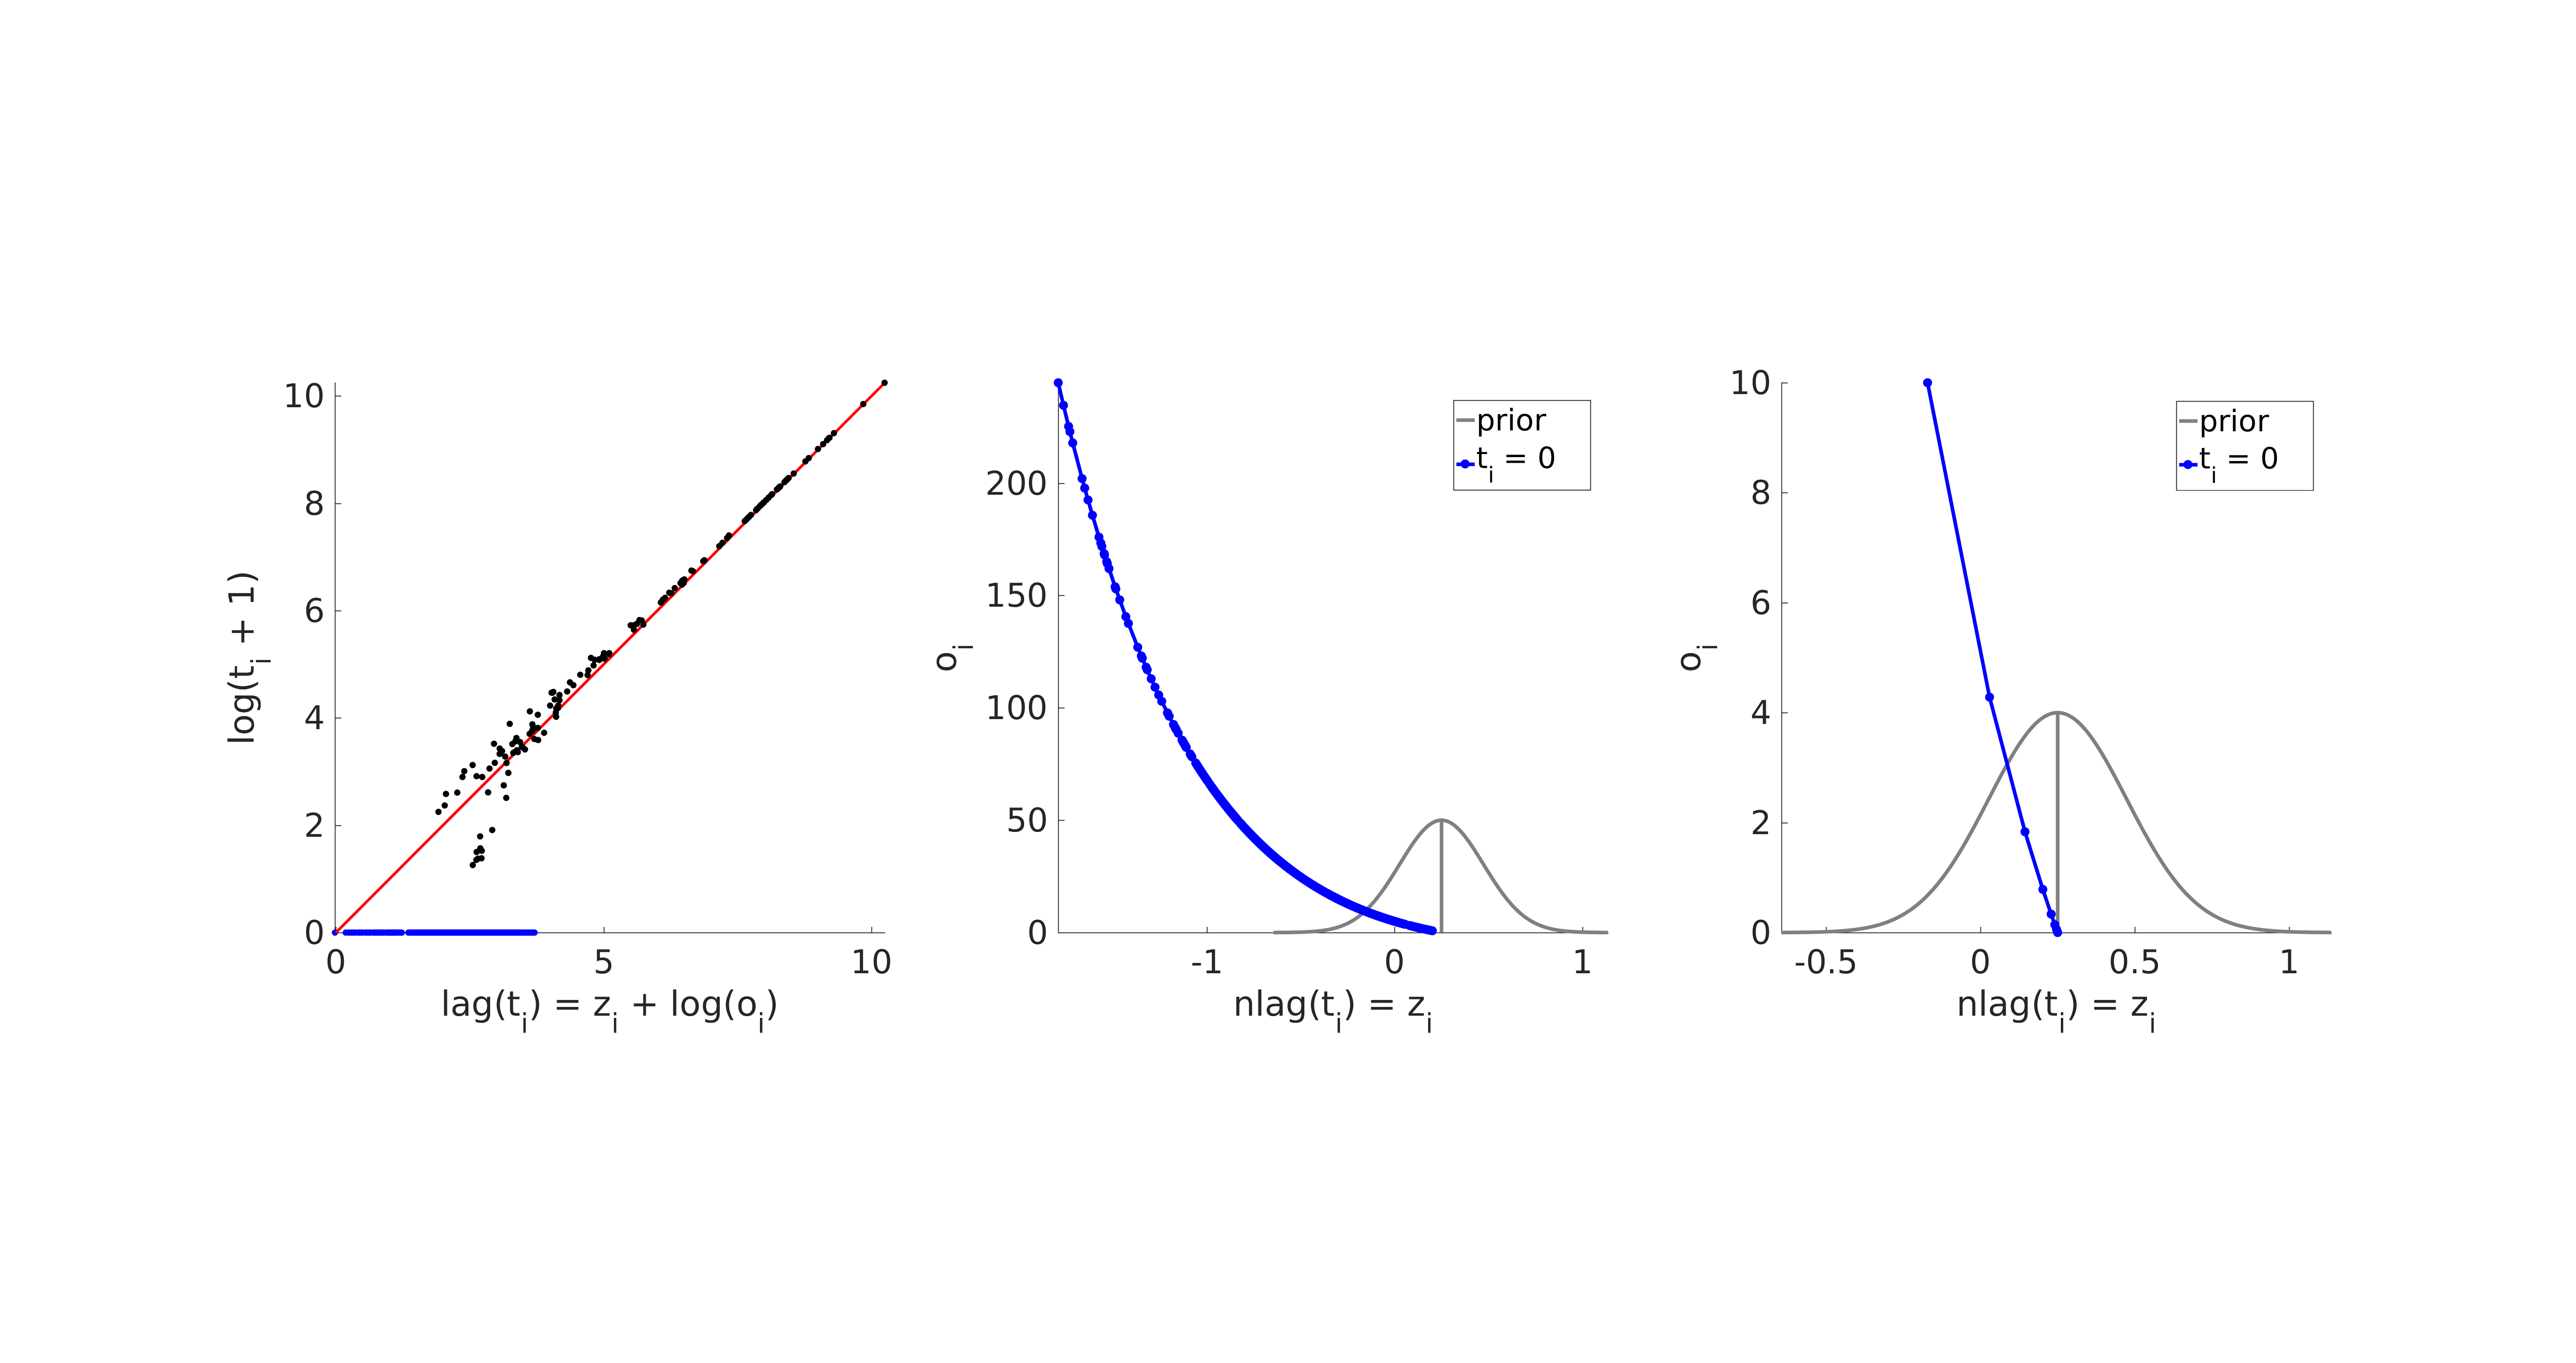
\includegraphics[trim={1cm 6cm 1cm 7cm},clip,width=\textwidth]{figure1.png}
\caption{}
\end{figure}




\end{document}